% This example An LaTeX document showing how to use the l3proj class to
% write your report. Use pdflatex and bibtex to process the file, creating 
% a PDF file as output (there is no need to use dvips when using pdflatex).

% Modified 
\documentclass{l3proj}
\usepackage{hyperref}
\usepackage{indentfirst}
\usepackage{graphicx}
\graphicspath{ {images/} }
\begin{document}
\title{Sports Facilities Management System}
\author{Atanas Pamukchiev \\
        Karl Drouven \\
        Dimitris Kiker \\
        Zoe Gerolemou \\
        Pedro Quintas\\
        Ross Imlach}
\date{March 27, 2015}
\maketitle
\begin{abstract}

The abstract goes here

\end{abstract}
\educationalconsent
\tableofcontents

%==============================================================================
\chapter{Our Project}
\label{ourproject}

%------------------------------------------------------------------------------
\section{Introduction}

\subsection{Preliminaries}

\par There are many sports clubs within and around Glasgow who offer coaching throughout the Summer. The latter run for a number of weeks and anyone interested in enrolling can do so for as little as a single morning, to several full-days of the week or, even, several weeks. For the purposes of this development, the attendance patterns are described in terms of sessions and blocks of sessions, where sessions are the events that actually take place, and are typically organised into blocks.

\par Most of the summer camps to date, utilise manual, paper-based methods for managing reservations. As a result, the retrieval and any later manipulation of bookings is extremely inefficient, increases labour costs, and acts as a bottleneck to the expansion of the relevant business venture.


\subsection{Aims}
\par
The primary aim of this project is to create a computerized booking and management system for Western Tennis Club, to improve the efficiency of the processes, and ultimately save coaching hours from waste. In addition, while focusing on the needs of Western Tennis Club, it is aimed to maintain reusability, so that the project can be easily adapted to the needs of another sports camp.
 
\subsection{Motivation}
\par
There are two key elements of high motivation in the project; the presence of an actual stakeholder underlies both. Being a project for a local business venture, its lifespan is expected to well outlast the duration of our studies, which entails the challenge of delivering a robust, well-engineered solution. Secondly, the fact that the requirements capturing occurs within a business environment adds a great challenge in the process, due to qualitative analysis involved.

\par In addition, another motivating factor is the challenge of developing and delivering software architectures, which are capable of adapting to unpredictable requirements (high modularity). The presence of the latter is the result of the adaptation to highly competitive environments, and unfortunately the cause of the writing off of many software developments. 


%------------------------------------------------------------------------------
\section{Our Stakeholder}
\par
The stakeholder for this project is the Western Tennis Club, part of the Western Health \& Racquets Club. This club is located in Glasgow’s West End, within close proximity of the University of Glasgow campus. Its facilities include a number of weatherproof and floodlit tennis and squash courts as well as a fully equipped, modern gym. The manager of the club, Julie Gordon, was in close collaboration with us throughout the duration of this project.
\par
The Western Tennis Club itself runs a number of programmes that aim to provide people with different sports backgrounds with the opportunity to either take up or improve their tennis skills with the assistance of qualified coaches. Lessons can be done in private or in groups, between players of equal level. The Club offers programmes that are suitable for both adults and children.
\par
Along with the regular tennis lessons, the Club also organises camps for children during the summer holiday period. The children can attend a single day session ( in the morning,in the afternoon, or both), book for a whole week or even book for more than one week. In addition to the tennis lessons and matches, a large number of different activities also take place in the summer camp, including football and rounder games.

%------------------------------------------------------------------------------
%==============================================================================
\chapter{Team Organisation}
\label{teamorganisation}

%------------------------------------------------------------------------------
\section{Model of Team Organisation}
\par
From all the team organisation models that are commonly used in the Software Engineering process, we chose to stick with the Role Based model. The Role Based model provides that the particular team that follows it is built around a set of roles which are either long-lived or created and assigned for a specific task (PSD3, 2014). We considered our organisation to be very flexible so that we have the option of having the different roles rotated within the team open throughout the whole project duration.
\par
The Role Based model that we used allowed us to provide the authority and responsibility for decision making to different people for different aspects of our project. We, of course, worked on a democratic basis, so each decision was taken after a group discussion between all the members of the team. In case of a disagreement between the members of the team during the discussion for making a decision for a certain issue, the person who was in charge for the specific area of the project was responsible for making the final decision as the most experienced and knowledgeable.
\par
When circumstances suggested so, we switched roles within the team in order to make sure we have a good fit for that role. In specific, when it became evident that the initially appointed project manager did not have the time to coordinate this project, resulting in organisational issues, the team underwent a project manager change. The most flexible roles such the Tool Smith and Secretary were undertaken by almost all the members of the team at different times.


%------------------------------------------------------------------------------
\section{Roles of Team Members}
\par
Our roles by the end of the project were:\\
\\
\textbf{Project Manager}: Dimitrios Kykeridis\\
\textbf{Chief Architect}: Atanas Pamukchiev\\
\textbf{Quality Assuror}: Karl Drouven\\
\textbf{Test Manager}: Pedro Quintas\\
\textbf{Customer Liaison}: Dimitrios Kykeridis\\
\textbf{Tool Smith}: Ross Imlach\\
\textbf{Librarians}: Pedro Quintas \& Zoe Gerolemou\\
\textbf{Secretary}: Zoe Gerolemou\\
\\
Each of these roles implied a set of responsibilities (PS3, 2014), listed below:\\
\\
\begin{itemize}

\item The \textbf{Project Manager} has the overall responsibility over the progress of a project and the organisation of the team and maintains the schedule of the project.
\item The \textbf{Chief Architect} is in charge of making high level design decisions for a system.
\item The \textbf{Quality Assuror} is responsible for assuring the quality of a software system and its documentation.
\item The \textbf{Test Manager} prepares the test plans and suites to evaluate the functionality of a project at different stages.
\item The \textbf{Customer Liaison} is the contact point between the software development team and the stakeholders and conducts all the in between communication.
\item The \textbf{Tool Smith} is in charge for the configuration and maintenance of all the different software tools used by the team and provides training on these tools’ interfaces to the rest of the team.
\item The \textbf{Librarian} prepares and archives the appropriate project documentation for all the different versions of a system.
\item The \textbf{Secretary} produces records of the project meetings and document them appropriately in order to be circulated to the other members of the team.

\end{itemize}

%------------------------------------------------------------------------------
\section{Team Communication}
\par
The team utilised different technologies available on the internet for internal communication. Each of the contact methods that were selected served different aspects of the organisation:
\\
\begin{itemize}

\item \textbf{Facebook Group:} The team set up and participated in a Facebook group that was used for both this project (TP3) and the Professional Software Development 3 (PSD3) project. Along with the Facebook Group, a group chat conversation was also created. They were used for arranging informal, day-to-day organisational matters quickly, such as deciding dates and times for our group meetings as well as the weekly supervisor meetings.

\item \textbf{Google Drive \& Docs:} These two services provided by Google were used intensively for keeping draft versions of documents to which all the members of the team needed to contribute. A folder was created and shared within the team in which all the documents that were products of collaborative work were stored. The members of the team took advantage of the concurrent access and manipulation that Google Docs offers for its documents to work on them in parallel.

\item \textbf{Github:} It was the web-based repository, and issue tracking service that we used throughout the implementation of our product. We have created a private repository on Github, that stored all the source code that our project comprised of, along with the final versions of our system documentation. We took advantage of the Version and Revision Control features that Github provides to work remotely and individually on the source code of our system.

\end{itemize}
%------------------------------------------------------------------------------
%==============================================================================
\chapter{Requirements Specification}
\label{requirementsspecification}

%------------------------------------------------------------------------------
\section{Research of Previous Products}
\par
Prior to the initial requirements elicitation, the team conducted a small research of previous products used within the industry for similar purposes. This was a crucial part of the preparation process since it provided an insight on how those systems are used and what features they provide. All of the above would be taken into account during the design and implementation of the new system. The following products were of particular interest to the team:\\

\begin{itemize}
\item \textbf{TennisBookingsPlus --- \url{http://www.tennisbookings.com/}}\\
A highly-customisable, web-based tool that enables Tennis Clubs to transfer their booking systems to an external web service that automates some of the clubs’ tasks. It provides a transition plan that helps their new customers to migrate to the new system. It provides features such as:\\
		\begin{itemize}
	\item Court Scheduling
	\item `Club New' Web Pages
	\item Online Payments
	\item Membership List Management
	\item Event Registration
	\item Online Bookings
		\end{itemize}
\item \textbf{TennisBiz --- \url{http://uk.thinksmartsoftware.com/}}\\
A very strong software package that administers both the class scheduling and the customer support using an integrated invoicing and marketing system. It is targeted for Tennis Clubs specifically, it is moderately flexible and configurable. It provides:
		\begin{itemize}
	\item Student grading system with respect to their skills level
	\item E-mail and SMS notifications system
	\item Attendance Tracking
	\item Waiting List for future enrolment
		\end{itemize}
\item \textbf{Bookingbug --- \url{http://uk.bookingbug.com/}}\\
A quite general booking system that can be used for scheduling various sports activities. ranging from sport club sessions to gym classes. The system can be personalised to meet the customers needs. Some of the features that it offers:
		\begin{itemize}
	\item Handling of Bookings, Appointments and Enquiries directly from the system’s website
	\item Online Payments
	\item Automated e-mail and SMS confirmations
	\item Calendar View for the Timetable
		\end{itemize}
\item \textbf{Teamer --- \url{https://teamer.net/}}\\
A flexible product that can be adapted appropriately for the requirements of different sports clubs. It offers a large range of different product variations to satisfy the needs of every customer. The purchase and installation costs for Teamer are very high compare to other products:
		\begin{itemize}
	\item Schedule Management
	\item Activities Organisation
	\item Online Payments (either deposit or full payment)
	\item SMS \& E-mail Confirmations
		\end{itemize}
\end{itemize}


%------------------------------------------------------------------------------
\section{Client Interview}

% - - - - - - - - - - - - - - - - - - - - - - - - - - - - - - - - - - - - - - -
\subsection{Preparation}
\par 
After conducting research on similar products, the team arranged a meeting with the stakeholder.  The purpose of this meeting was to capture the requirements for the new system. To achieve this, the team  prepared a number of different questions, designed to lead to useful conclusions, related to the design of the product. Their main aim was to warm-up the discussion and encourage the client to talk about how the summer camp is organised and describe their personal envision of the new system. In addition to the questions, the team prepared several User Stories and Scenarios that could help the stakeholder get a better understanding of the new system. These refinements were mostly done in order to remove any ambiguities or technical terminologies that might make the above documents unclear or difficult to understand for the stakeholder.

% - - - - - - - - - - - - - - - - - - - - - - - - - - - - - - - - - - - - - - -
\subsection{Provisional Interview Questions}
\par 

After careful consideration of the specifications, each team member proposed a set of questions to be asked during the interview. The final list of questions, as it was compiled before the Stakeholder Interview, can be seen below:

\begin{enumerate}
\item How are the classes set up?
		\begin{enumerate}
	\item Who plans the class structure?
			\begin{enumerate}
		\item Coaches, manager or both of them?
			\end{enumerate}
	\item How does the planning happen?
			\begin{enumerate}
		\item Coaches, manager or both of them?
			\end{enumerate}
	\item Are classes set up for people to enroll, or formed to meet the the demand post-enrollment?
\end{enumerate}

\item What is the registration process? 
		\begin{enumerate}
	\item Does the summer club use personal information forms already?
			\begin{enumerate}
			\item If so, could we please have a copy of the form.
			\item If not, then, could you please tell us what sort of personal information would you need from Parents and Coaches?
			\end{enumerate}
	\item To what extent is your system already computerised?
			\begin{enumerate}
			\item Is the information about the bookings held in electronic form? 
				\begin{enumerate}
				\item If yes, in which type of file? (e.g. a database, a spreadsheet)
				\end{enumerate}
			\item Have you been using any electronic booking management system, web-based or not? 
				\begin{enumerate}
				\item If yes, what problems have you faced during its use?
				\end{enumerate}
			\end{enumerate}
	\item During the registration process, are the Children able to register by themselves?
	\item Can parents enroll themselves to a class, too?
	\end{enumerate}
\item How many clients do you, roughly, have?
			\begin{enumerate}
			\item How many of them are registered for the winter sessions?
			\item How many of them just sign up for the summer camp?
			\end{enumerate}
\item How is the payment of the fees organised?
		\begin{enumerate}
		\item Is the full amount of money paid in advance or is it splitted into monthly (or other) installments?
		\item Do you keep payment information about customers after they have become your clients?
		\item Will customers be able to pay in cash at an office?
		\item Should the system include a client payment system?
		\end{enumerate}
\item How should the contact within the different users within the system work?
		\begin{enumerate}
		\item Could parent contact coaches or manager?
		\item Do we need an internal contacting system?
			\begin{enumerate}
			\item If yes, to what extent do we need implement it? (e.g. Just a contacts list provided to the users or implementation of a complete mailing system as part of the website)
			\end{enumerate}
		\end{enumerate}
\item Should we provide a customisable profile for the users?
\item Should the children have access to the system?
		\begin{enumerate}
		\item Should they access the system through their parent’s account?
			\begin{enumerate}
			\item If yes, should they access their parent's account with less permissions?
			\item If no, should we link their account to their parent’s one or just create a new, separate and completely independent, account?
			\end{enumerate}
		\end{enumerate}
\item Can children request to be with friends?
\item Should we include previous requirements that must be acquired by a player in order to be able to sign up for a class?
	\begin{enumerate}
	\item Are there any age restrictions to courses?
	\end{enumerate}
\item Should coaches be able to create and give awards to students?
\item Is the current manager keeping track of equipment and resources in venues? (e.g. balls, racquets)
	\begin{enumerate}
	\item Do you need an Equipment Report generated by the system?
	\end{enumerate}
\item What features are important to you? What would you expect to be able to do with the system?



\end{enumerate}

% - - - - - - - - - - - - - - - - - - - - - - - - - - - - - - - - - - - - - - -
\subsection{Meeting with the Client}
\par
The first meeting with our product Stakeholder took place on Wednesday, 22 October, 2014 in Room 303, the Triangular Meeting Room, Sir Alwyn Williams Building. Both our supervisor and our stakeholder attended the meeting.\\
\par Our Stakeholder is Julie Gordon and she is one of the coaches at the Western Tennis Club in Glasgow. She has been organising and managing the Summer Camp ever since its establishment.\\
\par After the team was introduced to the client by the Supervisor, the client was asked for her consent to record the discussion. Hence,  some general warm-up questions about the Western Tennis Club were discussed. The main objective was to encourage the Stakeholder to talk about the Club and its needs, before proceeding with more specific questions that may direct her responses. A lot of useful information regarding the operation of the club for both the winter and the summer seasons was gathered.\\
\par The complexity of our questions increased as the discussion progressed, in order to get more specific and detailed answers. At this step, most of the ambiguities were clarified.\\
\par Furthermore,  the electronic system that was currently used by the Summer Camp was examined in detail. The main focus were the personal details provided by the parents, in order to register their children in the Tennis Club and the storage and manipulation of the gathered data by the managers, in order to accept or decline the aforementioned booking.\\
\par At the end of the meeting, the team sincerely thanked the Stakeholder for her time and asked for her personal email address in order to set up a channel of direct communication between the Western Tennis Club management and the team. She was informed that via email she would receive the formal requirements specification document, produced after the end of Meeting, contacted for any clarifications around potential issues during the implementation of the project, and  asked to provide feedback for our product during the evaluation stage.
% - - - - - - - - - - - - - - - - - - - - - - - - - - - - - - - - - - - - - - -
%------------------------------------------------------------------------------
\section{Functional Requirements}
\par 
The requirements gathered from the meeting with the stakeholder suggested that the system should be available to three different kinds of users. To provide a better overview, each requirement is marked with a different user role, namely Manager, Coach, and Parent. Requirements that were role independent are marked with `For All Types Of Users'. When a Functional Requirement did not involve a particular kind of users but it was, mostly, related to the overall system, it was marked as `General'.
\begin{enumerate}
	\item \textbf{Creating Blocks \& Sessions (Manager):} The Manager of the Summer Camp should be able to create and set up new sessions,available for the children to be enrolled in. A number of these sessions will be combined together by the Manager to form a `Block of Sessions'.
	\item \textbf{User Registration (For all Types of Users):} A new user must be able to register in the system by filling in all the personal details required.
	\item \textbf{Child Registration (Parent):} Parents should be able to register their children, in order to enroll them in available sessions.
	\item \textbf{Making Bookings (Parent):} Parents must be able to view all available sessions, created by the Manager, for a specific child and enrol their children in sessions, by selecting different blocks of sessions.
	\item \textbf{Accepting a Booking (Manager):} The manager should be able to review, accept or reject new bookings. A booking should be considered as confirmed if the Manager approves it. Otherwise, if the booking gets rejected, it will be added to a `Waiting List'. 
	\item \textbf{Taking Attendance (Coach):} Coaches should be able to take attendance for all classes they are assigned to.
	\item \textbf{Making Payments (Parent):} Parents must be able to see outstanding payments and able to pay them in cash or online (PayPal).
	\item \textbf{Calendar View:} A calendar view of sessions could be a helpful feature for all users. For example, parents would be able to get a better overview of available or booked session. Also, Coaches and Managers would benefit from this feature, as it allows them to see assigned sessions or just get an overview of active sessions.
	\item \textbf{Game Scheduling using BTM Ranking:} The games between members of the Club could be organised automatically by considering their ranking by the Lawn Tennis Association (LTA). Players with similar rankings are believed to be of the same tennis skill level and could be placed in the same sessions to achieve higher learning outcomes for all members. The British Tennis Membership (BTM) ranking could also be used for scheduling matches between players.
	\item \textbf{Arranging coach payment:} The payroll for coaches could be generated automatically by the system and reduce the managers workload.
	\item \textbf{Internal Email System:} Internal communication between the different users of the system would be a useful feature. For example, managers could contact parents to inform them about problems related to theirs bookings. Furthermore, managers could also contact coaches to inform them about any changes to their assigned sessions. Also, parents could be able to contact the manager and arrange a meeting or request information.
	\item \textbf{Notifications for Payment Status:} Parents could be informed automatically by the system about the status of their payments (pending, due, completed), in order to assure that they are made properly and on time.
	\item \textbf{Preparation of Coaches'  Daily Plan:} Coaches could be able to propose plans for the assigned sessions through the system which then need to be approved by the manager.

\end{enumerate}


%------------------------------------------------------------------------------
\section{Non-Functional Requirements}
\par
Apart from the functional requirements the team defined non-functional requirements to describe more general attributes of the system rather than specific features. Non-Functional Requirements are defined to be the emergent properties of a system which cannot be tested by the presence or the absence of a feature (PSD3). \\
\\
The team defined the following non-functional requirements:
\begin{enumerate}
	\item \textbf{Flexibility:} The system should be flexible enough in order to be used by other sport clubs, without requiring extensive changes.
	\item \textbf{Extendibility:} The design and structure of the system should allow the implementation of extra functionalities in the future.
	\item \textbf{Portability:} The system must be available for different devices, including personal computers, tablets and smartphones. A mobile version of the Booking System will allow it to fulfill the `Strong mobile component’ requirement.
	\item \textbf{Security:} When deployed, the system will hold sensitive data, including contact details or medical conditions, for many users. Therefore, the data must be protected from unauthorised access.
	\item \textbf{Usability:} The system is targeted to be used by novice users. Therefore, the user interface should be intuitive and easy-to-learn.
	\item \textbf{Good Documentation:} The system will provide a large number of different features to all types of users. A user guide documentation should be provided with the final product. 
\end{enumerate}

%------------------------------------------------------------------------------
\section{User Stories}
\par
After the Functional and the Non-Functional Requirements of the system were discussed and decided on, the team compiled the corresponding User Stories, which were also provided to the Stakeholder along with the formal Requirements Specification Document.

\textbf{\underline{User Story \#1}}\\
As a \textbf{Manager}\\
I want to \textbf{create a new session,}\\
So that \textbf{children are able to enrol in them.}\\
\\
\textbf{\underline{User Story \#2}}\\
As a \textbf{Manager}\\
I want to \textbf{define blocks,}\\
So that \textbf{I will be able to group available sessions.}\\
\\
\textbf{\underline{User Story \#3}}\\
As a \textbf{New User}\\
I want to \textbf{be able to register to the webstie,}\\
So that \textbf{I will be able to use the booking system.}\\
\\
\textbf{\underline{User Story \#4}}\\
As a \textbf{Parent}\\
I want to \textbf{register my child,}\\
So that \textbf{I will be able to enrol them to a session.}\\
\\
\textbf{\underline{User Story \#5}}\\
As a \textbf{Parent}\\
I want to \textbf{be able to view all the available sessions for one of my children,}\\
So that \textbf{I will be able to enrol them to the sessions I prefer.}\\
\\
\textbf{\underline{User Story \#6}}\\
As a \textbf{Manager}\\
I want to \textbf{review a pending booking,}\\
So that \textbf{I will confirm it, in case I approve it.}\\
\\
\textbf{\underline{User Story \#7}}\\
As a \textbf{Manager}\\
I want to \textbf{review a pending booking,}\\
So that \textbf{I canwi add it to the “Waiting List”, in case I reject it.}\\
\\
\textbf{\underline{User Story \#8}}\\
As a \textbf{Coach}\\
I want to \textbf{take attendance for the sessions I am assigned to,}\\
So that \textbf{I will keep a record of the attendance.}\\
\\
\textbf{\underline{User Story \#9}}\\
As a \textbf{Parent}\\
I want to \textbf{be able to see any outstanding payment linked to my account,}\\
So that \textbf{I will arrange a cash payment for them.}\\
\\
\textbf{\underline{User Story \#10}}\\
As a \textbf{User}\\
I want to \textbf{be able to access a mobile-friendly version of the system,}\\
So that \textbf{I can access it from my mobile device.}\\
\\
\textbf{\underline{User Story \#11}}\\
As a \textbf{Parent}\\
I want to \textbf{be able to complete my payments online via PayPal,}\\
So that \textbf{I will not have to visit the Western Tennis Club each time I have an outstanding payment.}\\
\\
\textbf{\underline{User Story \#12}}\\
As a \textbf{User}\\
I want to \textbf{see available sessions on a Calendar,}\\
So that \textbf{I can organise my schedule easier.}\\
\\
\textbf{\underline{User Story \#13}}\\
As a \textbf{Player}\\
I want to \textbf{have my tennis matches arranged accordingly to my position in the LTA ranking,}\\
So that \textbf{I can play with opponents of the same tennis skills level as I am.}\\
\\
\textbf{\underline{User Story \#14}}\\
As a \textbf{User}\\
I want to \textbf{an internal email system,}\\
So that \textbf{I can contact other users within the system.}\\
\\
\textbf{\underline{User Story \#15}}\\
As a \textbf{Parent}\\
I want to \textbf{get notifications from the system regarding my payments,}\\
So that \textbf{I will be informed about their statuses (pending, due, completed).}\\
\\
\textbf{\underline{User Story \#16}}\\
As a \textbf{Coach}\\
I want to \textbf{submit plans for my assigned sessions in the system,}\\
So that \textbf{I will have it approved by the manager.}\\

%------------------------------------------------------------------------------
\section{Requirements Prioritisation}
\par After capturing both the functional and non-functional system requirements,  they were prioritised with respect to fundamentality and necessity for the product. The higher the priority, the sooner the requirement would be implemented, in order to ensure basic functionality of the system as soon as possible.\\
\\
The User Stories were classified in the following four categories: 
\begin{itemize}
	\item \textbf{Must Have:} Essential user stories that are required for the basic functionality. (Highest Priority).
	\item \textbf{Should Have:} User stories that are not essential for the basic functionality, but should be implemented in order for the system to operate properly. (High Priority).
	\item \textbf{Could Have:} User stories that are optional and not required for the basic functionality. The implementation of those should begin after completing the previous two groups. (Low Priority).
	\item \textbf{Would Like to Have:} User stories that are not planned for the iteration and beyond the scope of what is believed to be feasible (Lowest Priority).
\end{itemize}

{
\begin{figure}[h]
\caption{The Prioritisation of Requirements represented schematically}
\centering
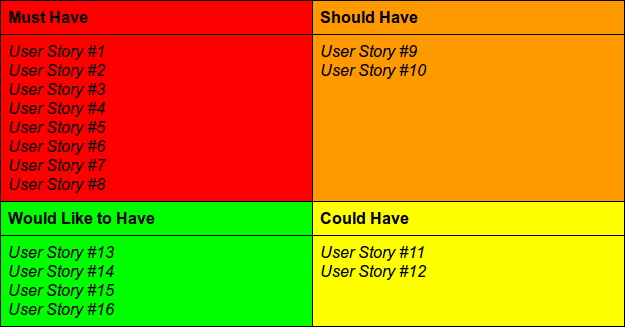
\includegraphics[scale=0.5]{Prioritisation.png}
\end{figure}
}

%------------------------------------------------------------------------------
%==============================================================================
\chapter{Design}
\label{design}

%------------------------------------------------------------------------------
\section{Managing Value}
\par
A user is satisfied by a system, if the system presents a high value for the user. That value must exceed the cost of doing so, and thus, the Booking and Management System had  to improve on and go beyond the functionality of the current system. Therefore, when designing the system, special attention was given to improving recurring tasks and providing defaults, where appropriately efficient. \\
\par First, the team focused on how to develop the Booking and Management System. Developing a web application was the most beneficial for a number of reasons. The alternatives were a desktop, an iPhone, an android and/or a blackberry application, increasing the development cost significantly. A web application allows access through multiple devices with a single implementation. It also assigns the complexity to the browser, rather than the operating system, allowing easier development, maintenance and deployability. The user does not need to download any software to use the system. A web application keeps all the functionalities for managers, parents and coaches in one single place, where all users, independent of their role, can login from the same page.\\
\par Hence, the team focused on how to display sessions and blocks to the user, and how to retrieve the editing of such bookings. The manager had to easily and intuitively create a new set of bookable sessions, yet allow for as much flexibility as possible. The current system had to be optimised, and the most rational solution was to allow the manager to create sessions, by inputting all the details for each session. However, as the new system would collect much more data for each session, the manager would have to fill in not only the details for multiple sessions daily, but also a larger amount of data. Hence, the manager would have to do more work than they usually have to, which was highly undesirable. It is important that the automation of such a process is flexible, in order to make the user engaged in using it. So the management of such cost and value is vital. The automation should also be accurate enough in order to actually increase the added value of using the product. This is why great care was taken to appropriately match the clients requirements and the tasks, accomplished by automation.\\
----------------------------------------
\par The sidebar allows the user to have access to all the functionalities, provided by the system. It also splits clusters of controls into an index of tabs, allowing for easier navigation. The starting `Overview’ page allows the high complexity of the system, and yet does not overwhelm the user. The most common tasks were included in the overview of each of the types of user. The manager `Overview' page displays the list of bookings pending confirmation, list of latest confirmed bookings, the waiting list of bookings and a list of members due to pay with a shortcut for printing. The parent `Overview’ page shows the list of payments due and the list of children. This means the user can quickly access the most important tasks. All other complex functionalities, such as lists of members and sessions, are kept in the sidebar for users who seek more information about the specific tasks.\\
--------------------------------------------
{\LARGE{EDIT HERE}}


%------------------------------------------------------------------------------
\section{Database Design}
\par
The Database design was the most challenging, time-consuming, and functionally important part of the project. In order for the team to be satisfied with the design and the planned functionality of the Database, a lot of improvement and refactoring was done on the initial versions until the final fully functional and practically implemented one was created. The process began with initial discussions of the functionalities to be supported by the Database. These discussions within the team aimed to clarify the precise proportion of the functionality to be built within the Database, in order to allow freedom and independence with respect to the type of sport. In other words, the team created a Database, which can fully support the management and booking system for any type of sport. The particular features to be deployed on the middleware were discussed as well. The following data was agreed on to be stored in the Database:
\begin{itemize}
	\item Personal Information
	\item Venue Information
	\item Group Information
	\item Event Details
	\item Payment information
	\item Login Details
\end{itemize}
\par In order to justify the team's decisions, the particular type of information within each data category used in the initial version of the Database are discussed.\\
\par 
Under `Personal Information' the database would store all the clients' and management's personal details, required for the normal operation of a sports camp, such as name, date of birth, email, and telephone number.\\
\par 
`Venue Information' would contain data about the venue, such as address, capacity, name, and load. Potentially, information about the venue’s manager might be included as well for larger scale applications.\\
\par 
`Group Information' would correspond to a coaching group, for instance, a class, and stores information such as capacity, the name of the group, the age classification, and, potentially, a human readable name.\\
\par 
`Event Details' would store data such as duration, any notes taken during that event, the group that is making this `event', and the venue at which this ‘event’ actually takes place.\\
\par 
`Payment Information' would include the amount of money due to be paid or paid already, the label, and the due date of the payment if applicable.\\
\par 
`Login Details' would store the passwords of the users.\\
\par 
This served as the first prototype of the database’s design and was extensively discussed among the team members and with the supervisor as well. The team faced a great challenge at this point since in order for the application to be as flexible as planned, a simple group-event relationship was not sufficient. Another level of complexity would be required in order for the Database (and respectively the Application) to be used by any type of camp. Furthermore, another difficulty emerged as the client demanded that the application had to distinguish between events in the morning and events in the afternoon, (as specified in Section 3.3 `Functional Requirements'). A sample solution, presented at a later stage, was able to partially solve the problem. The solution introduced some changes to the relationship between the future tables. `Group’s Events' became part of a sub-session, which is a part of a session itself. Those new terms were defined in the sense that events can be part of a sub-session, which in terms is part of a session. This way a session would have a location, but the sub-sessions of those sessions would be grouped according to whether they are in the morning or in the afternoon, and lastly events would have an associated coach capacity and group.\\
\\
{\LARGE{INSERT IMAGE}}\\
\par

This concept allowed a form of sub-classing, which solves the problem of the morning and afternoon events, since a sample database query would be able not only to get all the events as a part of a specific session i.e. define location, but also as a part of a specific sub-session, i.e. part of a specific part of the day.\\
\par This solution was, however, discarded as it would create too much redundancy within the database and only solved one of the problems present at hand. As the team continued to gain a deeper understanding of both the problem and the clients’ requirements, another Database refinement iteration had to be done, in order to optimise the kind of data stored and the way in which it was stored. Furthermore, several new tables were added to the prototype ER diagram. An important aspect of this change to the Database model was the addition of tables to store sub-venue information. This resulted in a redefinition of the term `Venue'. A `Venue' would now represent a real world address, being used by the company, operating the system. A `Sub-Venue', on the other hand, would now represent a facility, which is a part of that venue. A good example to illustrate this concept would be a club with address `1 University Avenue, Glasgow', say, with 6 tennis courts. This would be displayed in the database with one entry in the `Venue' table and six entries in the `Sub-Venue' table. In case the company starts operating another venue with address `2 University Avenue, Glasgow', say, it would be trivial to add this single entry. This feature was not a requirement of our client, but was added as it allowed the Database and the system to be used in companies of any size. The payment part was overhauled as well, including new fields that would aid the future application easily distinguish between pending payments and successful ones. Also, a distinction between the types of payments was included, since a PayPal payments feature was planned.\\
\par Following additional discussions within the team and with the stakeholder, even more features were added to the database. These included medical conditions records, the option to include extras in specific sessions, as well as taking notes and attaching them to specific sessions. Moreover, the Database could now store the BTM rank (or any other kind of rank) and the experience level of each member, so that filtration of the members could be done not only by age, but also by experience.  Of course the level would change, depending on the type of sport the application is deployed to interact with. A feature that was excluded was the storing of the login details, since the team figured out that Django can automatically handle and protect the login details,and therefore the corresponding tables became redundant.\\
\par However, at this time the Database Design did not fully solve the issue with the proper storage of the events information. The team continued investing time and energy in order to create a solution. Following numerous discussions and rigorous analysis of the issue at hand, the problem was resolved via abstraction of the events. The key element in this abstraction was the block. A block is a collection of sessions, which can have any attribute in common. This allows any kind of event to be easily distinguished and grouped by a common attribute. Hence, Events or Sessions can be grouped with respect to the time of the day they take place, i.e. morning or afternoon. Moreover, multiple sessions can be assigned to a single week or for the duration of a whole course. All of the features developed make the Database extremely flexible and hence, easy to implement in a system, dealing with any kind of sport or event.\\
\\ 
{\LARGE{DIAGRAM HERE}}\\
\\
\par In conclusion, the final version of the Database design provides multiple capabilities, some required by our stakeholder and others implemented in order to  serve other types of sports camps. \\

%------------------------------------------------------------------------------
\section{User Interface Design}
\par
Designing the User Interface began by planning and deciding on the priorities of the system. Since interaction with the clients is very important for a business such as the Western Tennis Club, the UI was designed with their needs specifically in mind. After the interviews and meetings it was clear that:\\
\\The `Parent' user had to be able to rapidly enroll a child into more classes, since this is the major driving force for the business.\\
\\The `Manager' user had to create a set of bookable sessions in a quick and efficient way. It would be an incredible workload for the manager, if every session they ever create is done individually.\\
\\The `Coach' user had to see its list of upcoming classes and check attendance for them.\\
\par Draft diagrams were sketched according to the Requirements Gathering and Prioritisation previously mentioned. Hence, they were reviewed by the team and further extended. These sketches are attached in Appendix A.1. This allowed for a better understanding of the system flow and any potential problems. During the interface design process, the team conducted extensive discussions regarding the display of specific functionalities.  It was decided that having a menu to travel through the different sections would be the most suitable choice, as it allows a quick outline of the functionalities, while giving the user an abstraction of each section. For example, the `Manager' user has multiple important functionalities available, such as confirming bookings and setting up sessions and blocks, etc. A navigation menu allows for these different functionalities to be displayed in appropriately aggregated clusters, and the user to see the available possibilities. If we have a menu button for `Members', the user knows right away that they can see anything related to members in that menu.\\ 
\par Another challenge was deciding on how to display the information in the best way. As the sketches show, the team had not yet decided about how to display the sessions and the the blocks to the users. Thus,, it was implemented very similarly to Western Tennis Club’s Google form (having checkboxes for each day of the week, representing mornings or full days). \\
\\ 
{
\begin{figure}[h]
\caption{Western Tennis Club Google Form}
\centering
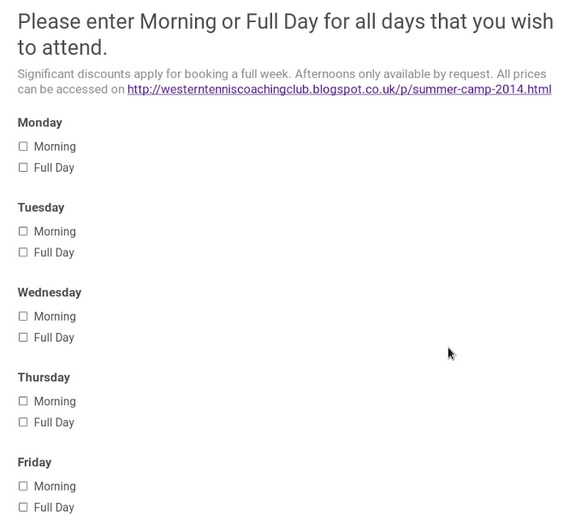
\includegraphics[scale=0.45]{googleDocsForm.jpg}
\end{figure}
}
\\
\par 
Since this system needed a mobile version, the UI was designed with that into consideration. Designing it for a mobile device allowed the website to be suitable for both small and big screens, since the smaller screen is the lower limit. After the general flow was established, a neater flow diagram of the system was produced for each user:\\
\\ \textbf{Parent: (Further designs can be found in Appendix A.2)}\\
{
\begin{figure}[h]
\caption{Parent View in Mobile Version}
\centering
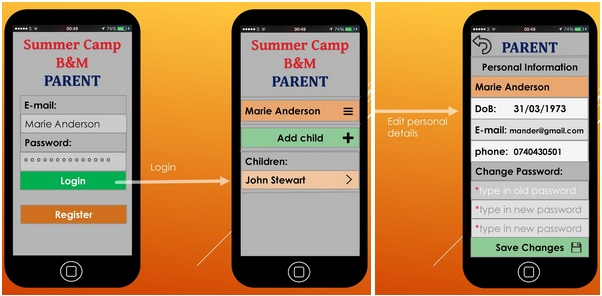
\includegraphics[scale=0.60]{diagramdraft2Parent.jpg}
\end{figure}
}
\\
\\ \textbf{Manager: (Further designs can be found in Appendix A.2)}
\\ 
{
\begin{figure}[h]
\caption{Manager View in Mobile Version}
\centering
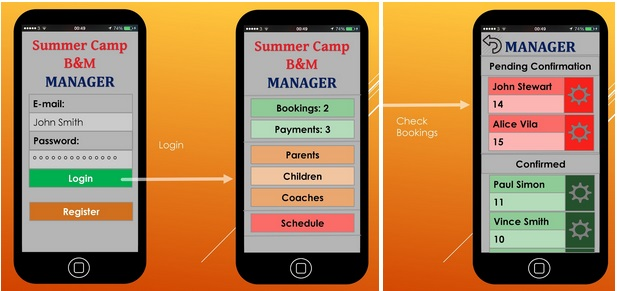
\includegraphics[scale=0.60]{diagramdraft2Manager.jpg}
\end{figure}
}
\\
\par 
Hence, this neater diagram was used to create the HTML templates. The templates were produced with hard coded data, to get the look and feel of the GUI to be consistent throughout the entire system. (More templates are attached in Appendix A.3)
\\ 
{
\begin{figure}[h]
\caption{Parent View in one of the earliest versions of the Booking Management System website}
\centering
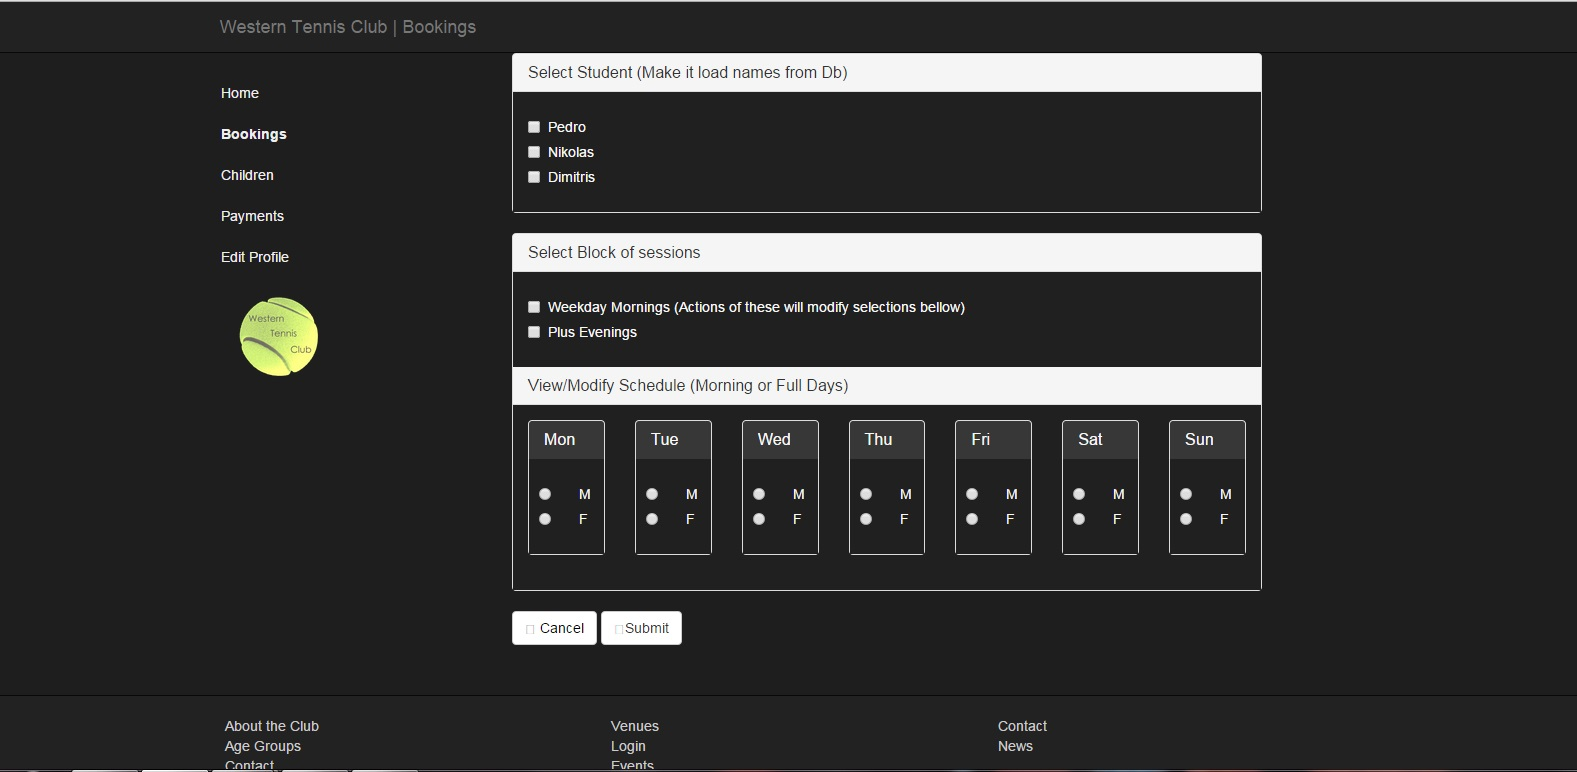
\includegraphics[scale=0.35]{parent_template.jpg}
\end{figure}
}
\\
\par 
The first template designs of the prototype were done in black and white to analyze the contrast better. Each cluster of controls are grouped into appropriate containers that allow for glanceable intuition. These served as the base for the actual implementation, giving the team a clear design style to follow and a common CSS style for the entire UI. This later led to the final Prototype:
\\ 
{
\begin{figure}[h]
\caption{Booking a Session (Parent View) in the Final Prototype}
\centering
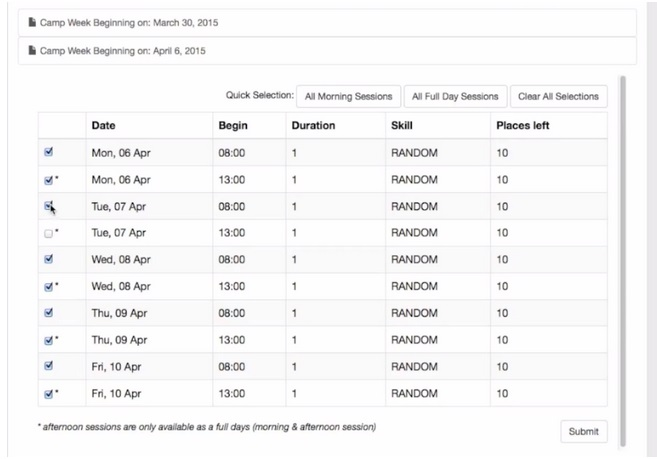
\includegraphics[scale=0.75]{parenttableFinal.jpg}
\end{figure}
}
\\
{
\begin{figure}[h]
\caption{Parent Overview Page in the Final Prototype}
\centering
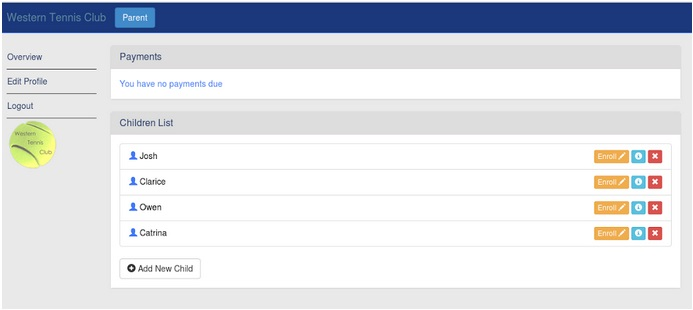
\includegraphics[scale=0.75]{parentlistofchildren.jpg}
\end{figure}
}
\\

%------------------------------------------------------------------------------
\section{Design Decisions}

% - - - - - - - - - - - - - - - - - - - - - - - - - - - - - - - - - - - - - - -
\subsection{Database Design Decisions}

% - - - - - - - - - - - - - - - - - - - - - - - - - - - - - - - - - - - - - - -
\subsection{User Interface Design Decisions}
The design decisions are crucial for the User Interface, since they define how the users interact with the system. Having the interface tailored for Western Tennis Club was an essential decision, since it allowed the team to personalize functions and defaults specifically to the client's needs. It was decided that having a news homepage was essential for the club to post potential news and promotions. Also, it was necessary to have different cluster of controls together in appropriate containers, so the user can distinguish between them at a glance. This menu was implemented as a sidebar instead of as a separate page, to allow the user to change between menus faster and with less clicks. The top navbar allows the user to keep track of where they are and if the screen is too small, the sidebar will turn into a popup sidebar, activated by a button, giving more space to the main display area. A footer was also implemented, so that the user can `contact' the club directly or read the `About Us' section. Below is a diagram of each of these areas. It was decided that the base HTML should be shared for the general outline of the design. Each type of user share an implementation of each sidebar. This reduces the amount of duplicated code and utilises any updates needed. Thus, any update or maintenance of the system becomes fairly trivial, due to the modularity of the UI.
\\
{
\begin{figure}[h]
\caption{Diagram that represents the Area allocation in the User Interface}
\centering
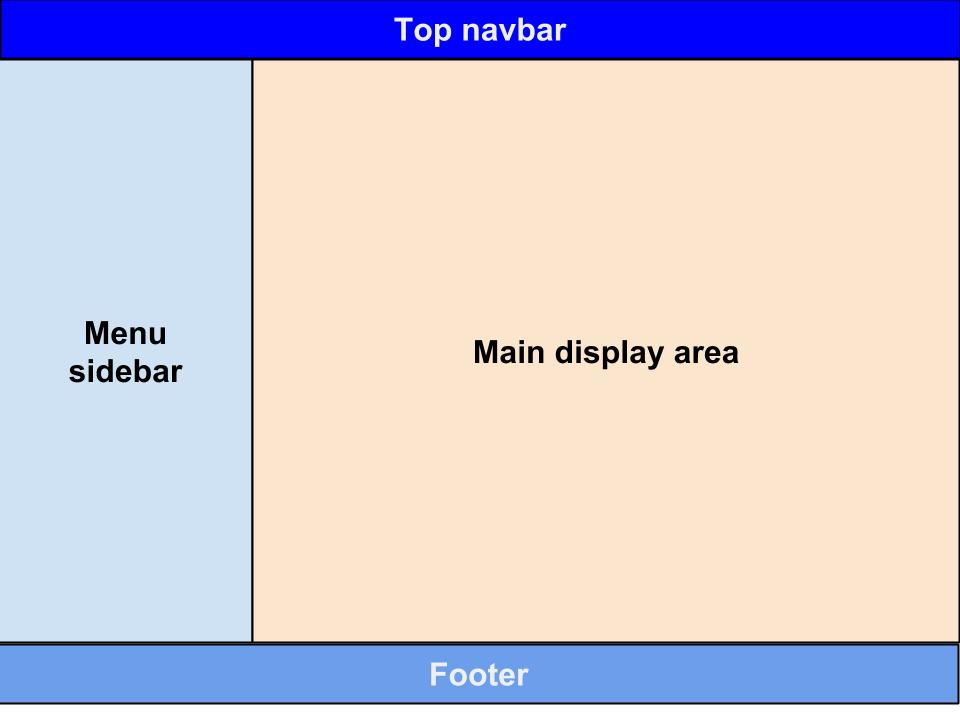
\includegraphics[scale=0.20]{AreaDiagramTP3.jpg}
\end{figure}
}
\\
\par It was decided that having the different clusters of controls, grouped by function, in dedicated containers would allow for glanceable intuition. Guiding the user through each section of controls such as the `List of Children' will show a parent a list of their children, with a button to add a new child, all inside a container of its own.\\
\par The colours were chosen carefully to give contrast between each cluster. On a projector having a lighter grey as the background would make it seem white, which in turn would dissolve the effect of the containers. On the initial HTML templates, mentioned in Section 4.3, the headers grabbed too much attention from the user. It was decided that having the body lighter would make it stand out, making it easier for the user to navigate through the system. The blue adds a theme to the organization, giving some colour without being emphasized. If the top bar was a stronger colour,  for example, red, it would detract from the emphasis the main display area should have. The header of each container is a darker grey with the purpose of giving the body of the container more emphasis. Where each button’s colour was chosen with respect to their functionality. For deletion and removal buttons, red was used to trigger warning. Blue is used for extra information, while orange is used to draw the parent’s attention to the enrollment. \\
\par The general look and feel uses Bootstrap's CSS library. This improves the system's flow due to the consistency of the different components used (such as text fields, buttons, tables and glyphicons). The icons were used to guide and help the users. They were chosen in accordance with the functionality at hand. For example, the remove glyphicon is used for deletion; the pencil glyphicon is used for bookings; the plus glyphicon is used for adding children. It makes the design more glanceable, rather than having each button tagged by text, and adds consistency to the overall look and feel.\\
\par Tables and list-groups are used to display lists of information. Tables are used only for a `Manager' user, as they display large amounts of data particularly well. Such as the list of members, blocks and sessions. List-groups were used where the user benefits from focussing on more specific data. Such as the list of children for a `Parent' user, where the attention should be draw to the name and the button controls on the right rather than their full details. For lists of pending bookings, it is clear that the attention is drawn to the control buttons, since dealing with bookings is the main focus of that panel. The list of coaches, for the `Manager' user, extends down a list of users to be given the privileges of a coach. The list has a search filter and because it extends, when the user clicks the `Add Coaches' button, it draws their attention.
\\
{
\begin{figure}[h]
\caption{List of female members for the Manager View}
\centering
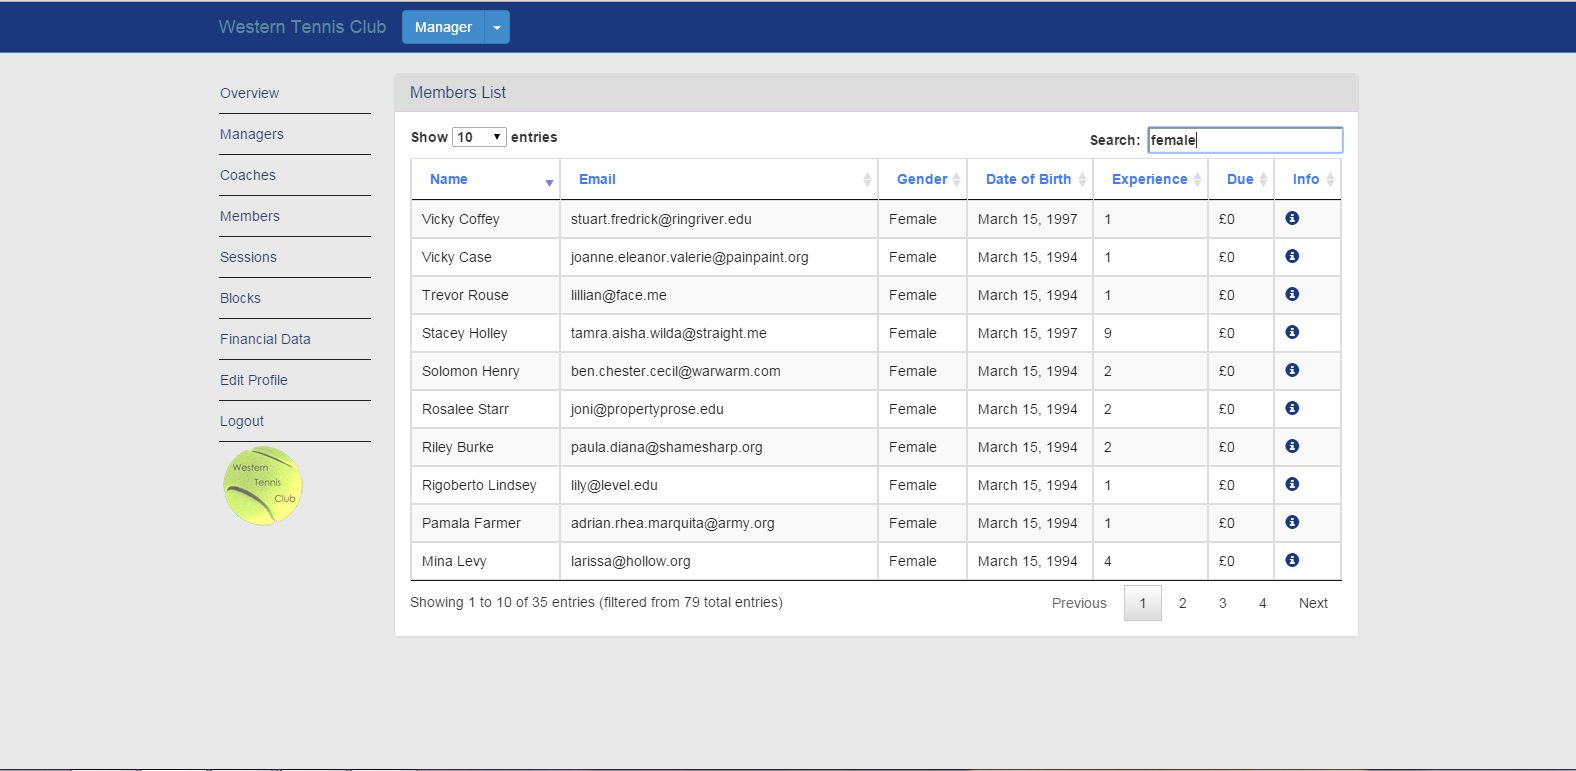
\includegraphics[scale=0.40]{managerlistofMembersFemale.jpg}
\end{figure}
}
\\
{
\begin{figure}[h]
\caption{Manager Overview Page}
\centering
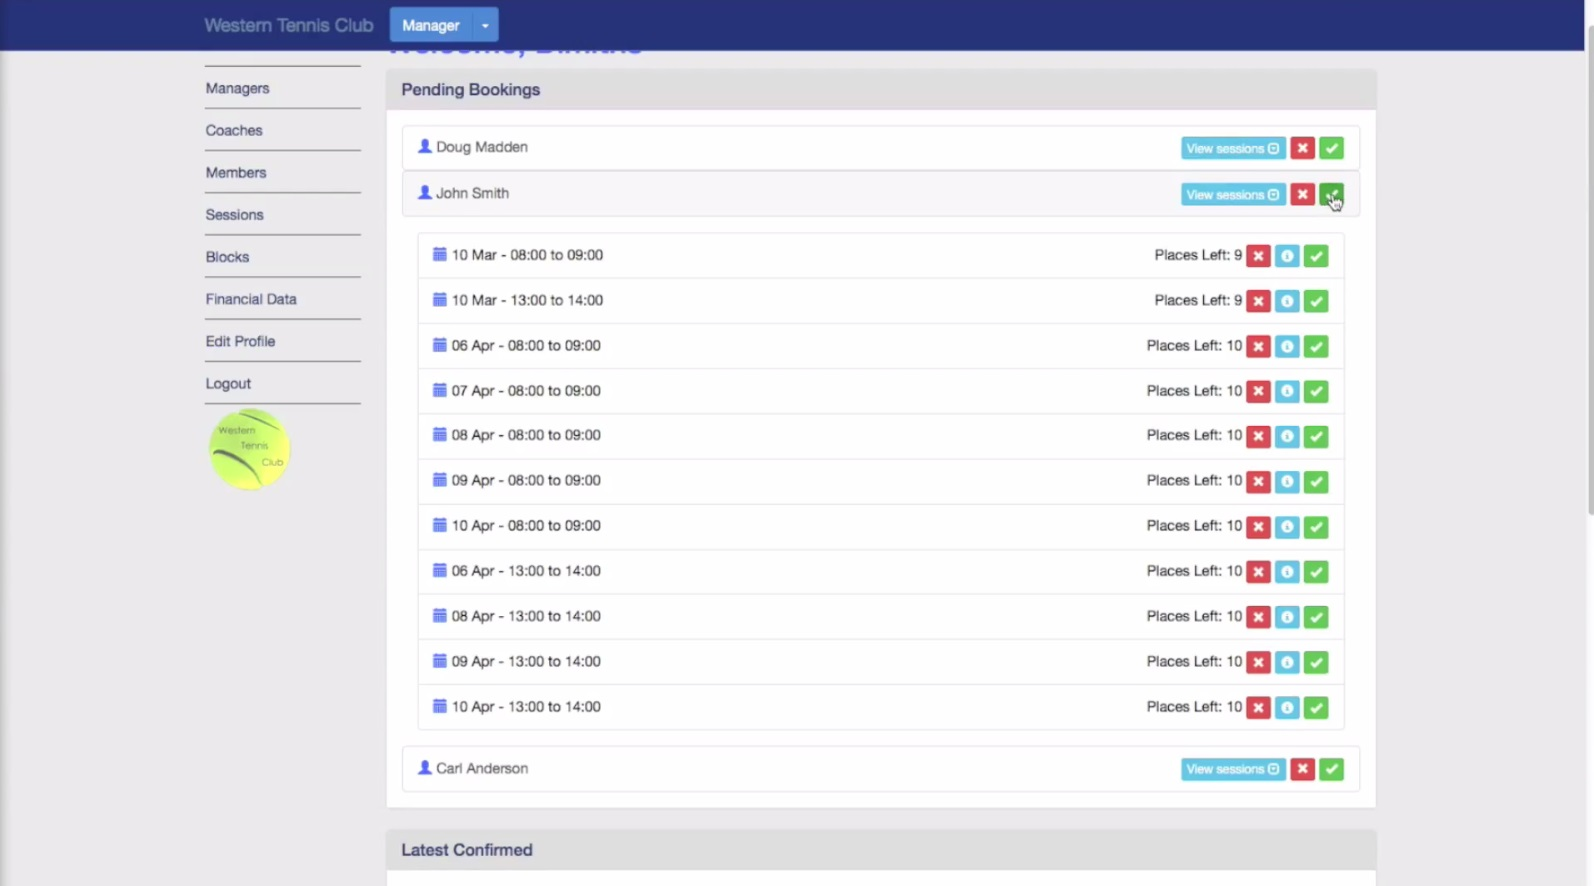
\includegraphics[scale=0.30]{managerOverview.jpg}
\end{figure}
}
\\
{
\begin{figure}[h]
\caption{Adding a Coach in the Manager View}
\centering
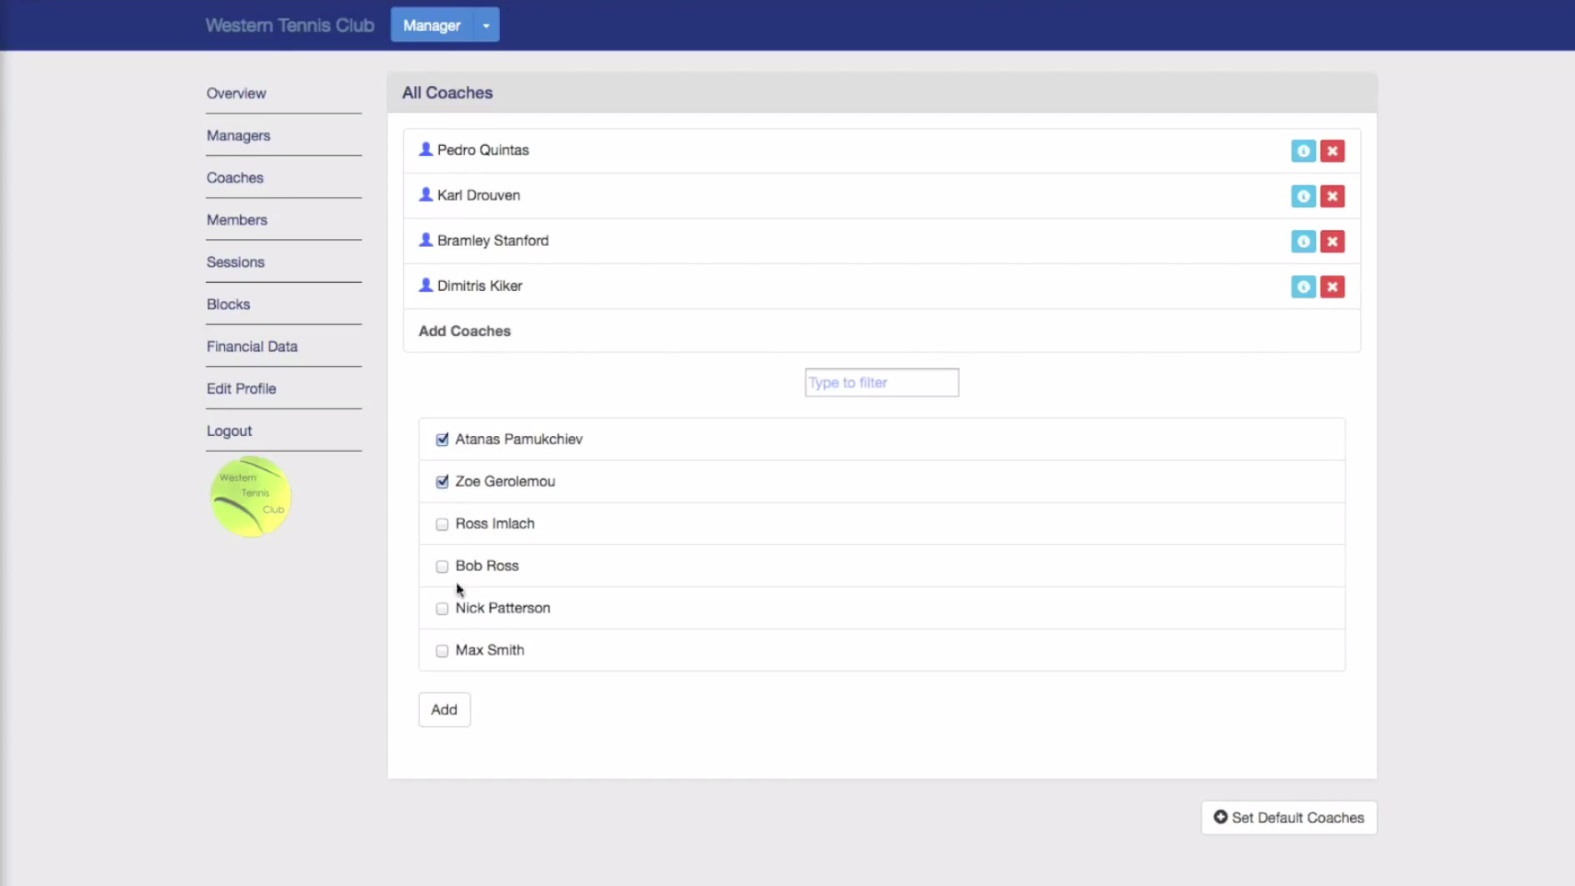
\includegraphics[scale=0.30]{managerCoachList.jpg}
\end{figure}
}
\\
\par 
The three different users were handled by a flag, that grants access to a `Parent', `Coach', or`Manager' user. Anyone who registers, gains `Parent' access status automatically. Then they can be upgraded to coach and/or manager by another manager, in the list of coaches and managers accordingly. All of these details were chosen with the specific client in mind.\\
\par An important issue that was raised during the design of the system was how the parents will accomplish the booking of the desired sessions for their children. Since the bookings are one of the main features that the system has to offer, any design decision that is related to this, was considered as crucial. There were two different perspectives on this issue within the team. The former stated that all the sessions should be predefined, in advance, by the manager, leaving the parent with no other option but selecting one of these blocks. The latter provided more freedom in the block selection since it allowed the existence of both predefined, but also customisable blocks that would be created by the parent on the booking time. After an extensive discussion, where the pros and cons of each option were presented and weighted, and by taking the  Supervisor's advice into consideration, it was decided that the system would offer both predefined and customisable blocks for booking but to handle different bookable periods within the Tennis Club. The predefined blocks would be used to organise the classes that run throughout the winter period and the customisable ones to manage the Summer Camp Weeks. The flexibility that the customised blocks offered seemed more suitable for the Summer Camp period when the parents want more freedom on preparing their children's schedule. In contrast, the parents want more consistency on their children's timetable during the winter, because they need to arrange their schedule appropriately to serve both their family and work commitments.\\
\par A big focus was put on automating recurring tasks and improve their efficiency. Gathering feedback from Western Tennis Club allowed for tailored defaults to be set to increase the automation of tasks. For a manager to create a week of camp merely two fields are required (a starting date and a name label). The morning and full day approach to bookings was designed and improved by checkboxes with default selection buttons for enrollment for a `Parent' user.\\


% - - - - - - - - - - - - - - - - - - - - - - - - - - - - - - - - - - - - - - -
%------------------------------------------------------------------------------
%==============================================================================
\chapter{Implementation}
\label{impl}
The implementation process began after all the design decisions had been completed. During the implementation it was very important for the team to receive as much feedback from the client as possible in order to achieve a product that meets the clients expectations. To accomplish this, a simple prototype consisting of example HTML files and CSS files was developed to present to the client. After receiving the client feedback, the actual implementation process began.

To allow this process to be completed in a timely manner, the system was divided into sections; front-end, back-end, database and security. Each team member was assigned  at least one of the sections in order for the work to be done on each section simultaneously and enable individuals to focus on one specific part of the implementation. The specialisation of each team member lead to a higher quality of the overall implementation.

Most team members had never developed a web application of this size before, therefore the team decided to choose software tools for each section that used programming languages and concepts which the team was familiar with and were also well documented. These choices were also influenced by the time constraints of this project.

%------------------------------------------------------------------------------
\section{Project Setup}
{
\begin{figure}[h]
\caption{System Structure and its targets}
\centering
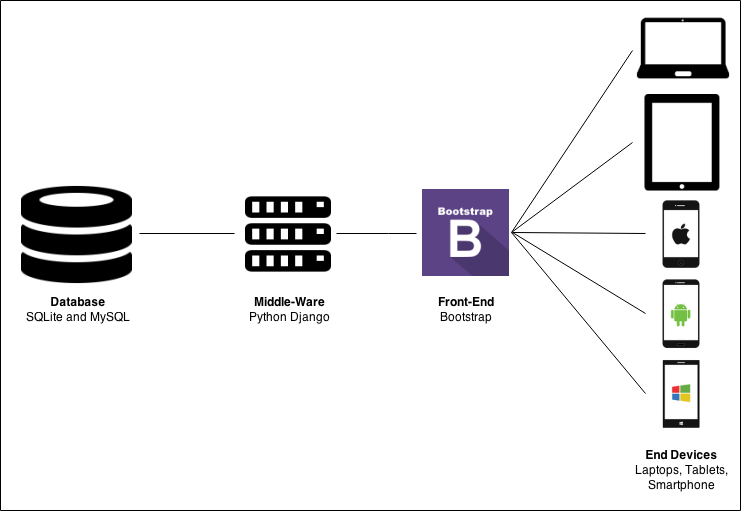
\includegraphics[scale=0.28]{SystemStructure.png}
\end{figure}
}
%------------------------------------------------------------------------------
\section{Front End}
\par
As previously mentioned, the stakeholder had some requests for the new implementation of the front-end. The user interface should be highly user-friendly and allow the user to complete their tasks efficiently and without distraction from unnecessary information. It should be consistent, modern and convey an overall professional look. The final request was that the user interface should be responsive so that the user can access the web application from different devices, including laptops, tablets and smartphones, whilst still allowing high usability.\\
\par To meet the stakeholders request to build a responsive and user-friendly web application, the team decided to use a front-end that was especially designed for this purpose. Bootstrap and Foundation are the two most popular frameworks that were designed for mobile first projects and therefore ideal for this project. In addition to being responsive frameworks supporting all standard browsers, an extensive library of user interface components like buttons or glyphicons are available. Due to their wide use and popularity, most users should feel familiar with the components, which makes the web application more intuitive.\\
\par Although Bootstrap and Foundation appear to be very similar, there are some differences between them. For example, Bootstrap allows customisation of the visual appearance, however, Foundation performs slightly better in this task and allows developers to eliminate the default look. Bootstrap, on the other hand, is intended to create web pages as efficiently as possible and therefore allows quicker deployment.\\
\par Most comparisons on the internet conclude that the decision for one of those frameworks should be made on personal preference since the basic functionality of both frameworks are the same. In the end, the team decided to use the Bootstrap framework, as it is the more popular choice amongst web developers and one team member had used it in a previously and was able to assist other team members.\\

%------------------------------------------------------------------------------
\section{Database}
\par As discussed in the design section above, it is clear that the database is a very important part of this project. The database is responsible for storing and organising data that is used by the web application. The Django back-end framework is able to use three different database systems; MySQL, SQLite and Postgres. All of those support the basic SQL functionality, however, the team was looking for a database that could be deployed without too many difficulties and too much maintenance during the implementation process. Initially the team planned to use MySQL because it was supported by Django, was scalable and secure and was also the DBMS with which the team was most familiar with. But when the application was first deployed and started a problem was revealed. There was no efficient way for the team to synchronize the development database between their computers and to be able to rollback any changes made to the information in the DB.\\
\par After some research, the team decided to use the SQLite database because of the fact that it is a lightweight fully functional SQL database engine. The entire database is self-contained in one single file and does not require an additional server processes, configurations or maintenance to operate. It can be directly integrated into the Django back-end which is also important at the development stage of the product. However the team would suggest that the Database back end be changed to a more scalable and robust DBMS, because of the metrics collected during the evaluation sage. Those metrics suggested that when the system is extensively used the back end could get as many as thousands of hits per second, and this could be a problem for a back-end such as SQLite which is not that scalable. The final web application is planned to be a medium traffic website that will receive 500 - 1000 HTTP requests that include dynamic content in a typical day. SQLite states that the database engine is able to deal with about 100,000 hits per day without any disturbance and therefore for an initial deployment such usage intensity would not be a problem. Furthermore the maximum capacity of the database is far above the minimum requirements of 10 giga-bytes that were set by the team during the design steps. Finally the last reason to choose SQLite was the fact that a migration at a later stage to a different DBMS would not be a problem since it requires only a couple of changes.\\
\par Because of the initial choice of MySQL as a DBMS the first database was created using MySQL’s schema creator. The schema itself was discussed in the database design section and its actual creation was even easier because of the graphical relation builder that MySQL provides. Later it was easily migrated to the server using the built in migrator and the local server started. Because of the already discussed problem with the data not being easily accessible between multiple development machines the same MySQL schema was translated to SQLite using a script and the database file was added to the project folder.\\
\par 
Even though the database was deployed already during the implementation process there were a number of cases which required columns to be added or removed or even data types to be changed. Because of the fact that the team would already be well into the development process the changes introduced had to have minimal effect on the rest of the structure. A good example of this was the fact that the team did not include an isMember boolean field to the client details(Which was required by the client). Because of the fact that this field would be required for every user and the  way django models work such an addition required the whole existing database to be dropped and rebuilt. Such a task can waste a lot of time and was a serious mistake made during the design stage. Another change that was introduced at a later stage involved the addition of a separate table to hold parent’s telephone numbers. The reason for such a change was lack of understanding of the way django works. The current model as described in the database design section uses a combination of the tables of the team’s database and the django required database. Because of the fact that parent’s details are stored in the django generated part of the DB they simply cannot be changed once the application is started and deployed because the cost of doing so is enormous. This is why the team came up with a solution that simply added a separate table to store the telephone numbers of users. This required a bit more server side work in order to make sure that this field is also populated when for example a new user is registered. \\


%------------------------------------------------------------------------------
\section{Back End}
\par
As discussed before, the team decided to implement a web application. The three most popular web application frameworks at the time were Ruby on Rails, Flask and Python Django. Similarly to the front-end frameworks, all three back-end frameworks offer the same functionalities, but differ in their implementation. Most developers will therefore base their choice of framework on their preferred implementation style.\\
\par 
Most team members had no previous experience with web development so the first instinct was to look for a framework that was easy to learn and did not require much configuration. Ruby on Rails was the first framework on the teams research list, as it is famous for offering many default settings and therefore allowing quick deployment. Furthermore, it follows many software engineering patterns such as `don't repeat yourself', `Batteries included' or `model-view-controller', which most team members were familiar with already. Unfortunately, Ruby on Rails is written in Ruby and no team member had used this language before. Due to the time constraints of the this project, the team did not have the ability to learn a new language, so the team decided to continue the research with the other frameworks.\\
\par 
The next framework that the team took into consideration was called Flask. Like Ruby on Rails, it comes with many default settings, which allows a quick deployment of the framework. Furthermore, Flask is written in Python and is described as ideal for inexperienced web developers. All team members had used Python before which meant that this feature would help to speed up the implementation process and finish the project in time. Unfortunately, Flask is not designed for medium scale web applications as required by the team.\\
\par 
The last web application framework on the teams list was Python Django and like the name suggests, it is written in Python. It is used by large scale web applications such as Instagram and Pinterest and therefore suitable for this project. Compared to the other two frameworks, Python Django offered high customisability, which meant that it could not be deployed as quickly. However the team preferred to implement a framework that could be tailored to the requirements rather than have limitations during the implementation. Furthermore, Python Django is famous for allowing rapid development, which has been a constant concern in this project, since the team decided to build a complex web application in a short period of time. The framework also supports software engineering patterns like `Batteries included' or `model-view-controller' which allowed a more independent implementation. The web application will hold a lot of data and that is why the team was looking for a framework that offered a simple connection to the database. Python Django can be easily extended with MySQL, Postgres and SQLite and offers a better interface to the database then the other two frameworks. The framework is able to automatically create new tables in the database and data through defined models in the framework, meaning that no SQL code is required.\\
\par 
After some discussion, the team decided to use the Python Django framework. It may not be the most popular choice between those three web application frameworks, however, it offered very well written and extensive documentations which was important as most team members had never done web development before. Also, the recommendation to use Python Django by one team member reaffirmed the decision made. The next important decision to be made was what version of Django should the team select. At the requirements capture stage the latest stable release was Django 1.5.4. The release candidate was Django 1.7 and it offered some security improvements and also database migratability. The main problem with the newer version was the fact that it was not widely used (and bug free) and therefore the team chose 1.5.4. 

%------------------------------------------------------------------------------
\section{Security}
Throughout the entire implementation process, security was a major concern to all assigned team members. When the system is deployed, it will hold sensitive data such as contact details and medical conditions. Such information is often targeted throughout the internet and this is why extra precautions were taken during the implementation of the back-end and database. It is important to note that the team had almost no experience with the security aspect of web development and therefore all the precautions that were taken were purely based on additional research and also some very helpful workshops hosted in the University of Glasgow which were targeting security in the web.\\

\subsection{Back-End}
The Django back-end already has some security features built in to help developers reduce the risk of a breach in security. Additionally, the documentation covers extra techniques that should be used during implementation. Before the implementation process started the team discussed several security issues related to the back-end and tried to take them into consideration during the process. These included:\\
\par 
The user authentication system provided by Django was one feature that helped the team to achieve high security standards and also to speed up the implementation process. Without any complex configuration the system was able to deal with user accounts, account passwords using hashing and salting, group permissions, general permissions and cookie-based sessions. The individual team members working on this part of the implementation were able to make changes to the system to comply with the design decisions made before. This feature protected the entire web application from unauthenticated users.\\
\par 
With the help of \underline{django.auth} three user groups were defined, and all the users created with help the authentication system are assigned to one or more of those user groups. This feature allowed the team to restrict web pages to specific users who were not authorised to view them. For example, only users that are in the Manager group are able to access manager tagged web pages. However, if a user tries to access a page without their restricts, they are automatically redirected to their index page. \\
\par 
Another important security improvement is concerned with data communication within the app through the links. This is an easy way of communicating information between different views by sending some information via the url. On the other hand it is not as secure as using, for example communication through the built in Django, context feature.For example, if the user would like to see their child’s profile the user clicks on a link that may look like this:\\
\texttt{http://...domain name…/bookingsystem/parent/childProfile/6}

The last digit in the URL is the child’s User ID in the database. To avoid parents opening another user’s child's profile by changing the last digit of the URL the team members implemented extra security steps that guarantee that the request child belongs to the authenticated user that requests the profile. This principle is used in other sections of the system, for example for coaches that access their timetables.
\\
\par Also, Cross-Site Request Forgery protection and Form Validation were used to protect the communication between the users browser and the back-end. CSRF protection is supported by Django and was enabled to work with the built in cookie management which is responsible for keeping track of active users and protecting the sessions of those users from attacks. Forms on the other hand were implemented so that they include the built in data validation as well as additional protection using custom validation that makes sure the data submitted is appropriate and that no attacks such as SQL injection can occur.

\subsection{Database}
\par
The current implementation of the database does not support any encryption or password protection. However, as previously mentioned, the team was looking for a database that was easy to deploy and required as few configurations as possible in order to finish the project. To increase security before the actual deployment of the system, the team strongly suggests to migrate the SQLite database to a database system that supports higher level of security like MySQL.

%------------------------------------------------------------------------------
%==============================================================================
\chapter{Testing, Evaluation and Future Improvements}
\label{testevfutimprv}

%------------------------------------------------------------------------------
\section{Testing Procedure}
Throughout the development lifecycle, test procedures were followed to ensure that all operations led to the desired result. Extra precaution was taken for operations that involved manipulation of the database, as those might cause data to be incorrect or corrupt.\\
\par 
After a team member completed a new feature, it was extensively tested with sample data that was stored in the database. Additional records were added to the database if they were required to test the new features.\\
\par Apart from specific testing, black box testing was used several times during the development lifecycle to ensure that all individual implemented parts were working together as a complete system. The two most extensive black box tests took place before before the first client evaluation meeting to ensure that the client could use it without facing any errors and after completing the implementation process to make sure that it meets the Western Tennis Club requirements. 

%------------------------------------------------------------------------------
\section{First Client Evaluation Meeting}
As soon as the primary functionalities of the system had been implemented, the team decided to arrange an evaluation meeting with the stakeholder in order to receive feedback and make appropriate changes to the implementation.\\
\par 
During the meeting the stakeholder was walked through the web application as all types of users, in order to understand the process that had been made at that time. Furthermore, this procedure encouraged the stakeholder to see potential problems and recommend enhancements or corrections that would improve experience for potential users.\\
\par 
After the demonstration, the stakeholder, Ms. Gordon, congratulated the team on the progress and was able to give some feedback. For example, users should receive an email confirmation after registering to the system, when bookings are confirmed and payments have been accepted. The stakeholder also suggested an SMS notification system in order for parents and coaches to be informed about last minute changes. After some discussion the team and the stakeholder agreed on an implementation of an internal email system which allows more flexibility and less maintenance.\\
\par 
Another feature that the stakeholder suggested and considered to be extremely useful was a search and filter option for different parts of the system. For example, the manager should be able to find members from a list by simply typing in some letters of the members name. This should improve usability as the manager would not require to scroll through an endless list of users.\\
\par 
Later, the team discussed features related to the Tennis Club management. The client clearly prefered the ability of adding new venues through the system over having all the available venues hardcoded in the Database. Furthermore, she proposed some changes to be applied on the way the children's personal details are handled by the system. Instead of storing the current age for each children, she suggested that it would be better to replace it with their Date of Birth. That would lead to more convenience when dealing with the allocation of children to their appropriate age groups. Additionally, she considered as urgent to have the medical condition field completed for every child in the Club so that the coaches would be totally informed about their trainees.\\
\par 
A number of suggestions made by Ms. Gordon were related to the payments feature. She believed that this functionality had to be extended to several other aspects so that it satisfies the Tennis Club needs as much as possible. The system ought to allow both full and partial payments, depending on client's preference. As soon as a new payment was completed, either online or cash, the system should update the corresponding record, immediately, to prove its responsiveness and avoid any misunderstandings on upcoming transactions. Additionally, she proposed that it would be very convenient if the coaches' payment would be fulfilled by the system itself. Any level of automation in the payment seemed to be extremely appreciated.\\
\par 
By the end of the meeting the team had a clearer view on the client’s requirements for the system. Hence, the team was ready to proceed with the implementation in accordance to the guidelines given.




%------------------------------------------------------------------------------
\section{Final Client Evaluation}
For the final client evaluation the team decided to allow the stakeholder to try the web application without interference from team members that might influence the opinion. At that point the system had been extensively tested in order for the stakeholder to experience how the final product will perform.\\
\par 
To allow the stakeholder to access the web application and interact with it, the team decided to host it on PythonAnywhere, which is an online integrated development environment. To provide some guidance the team created an evaluation sheet that included common tasks for all types of users. The link and the evaluation sheet was sent to the stakeholder with the request to try out the web application and sent back the completed evaluation sheet.\\
\par 
The feedback received from the stakeholder commented on the efficiency of the system and the performance of individual tasks. The overall feedback was positive and included comments on the high performance and high potential of the system. The stakeholder also included suggestions for further improvements. For example, the system should have a better error prevention and handling and even less data input repetition.\\
\\
The received feedback was very useful for the team and will be taken into consideration for future improvements 
%------------------------------------------------------------------------------
%------------------------------------------------------------------------------
\section{Heuristic Evaluation}
Apart from its performance, the Booking Management System deployed was also evaluated for the design of its User Interface. Jakob Nielsen's \emph{Heuristics} (Nielsen, 1994) was the set of usability heuristics that were used to review the User Interface:\\
\\
\textbf{Visibility of system status:}
The system keeps the Users informed about its status with the appropriate messages that appear within reasonable time. Whenever a task is completed, the system returns the corresponding `Successful!” message to mark this accomplishment.\\
 \\
\textbf{Match between system and the real world:}
The System uses words that are familiar to the Users such as ‘Coach’, ‘Sessions”’ and ‘Enrol’, whilst it avoids technical terms and notions that may be unknown.\\
 \\
\textbf{Consistency and standards:}
The same words and icons are used throughout the system to mark the same operations. For example, the X icon is used everywhere to mark the deletion of a User (either a manager, or a coach).\\
 \\
\textbf{Error prevention:}
Most of the operations that are done via the System require a confirmation before they are completed; especially the ones that perform deletions of Users or Sessions. They are used to prevent any errors that are caused by Users when they accidentally, commit an action that they do not intentionally want to.\\
 \\
\textbf{Recognition rather than recall:}
All the objects and icons throughout the system are clearly visible so that the User does not have to memorise a process simply recall it.\\
 \\
\textbf{Flexibility and efficiency of use:}
The System design allows the common tasks to be no more than three clicks away from the User in order to accelerate the process and save time.\\
 \\
\textbf{Aesthetic and minimalist design:}
The System’s design is fairly minimalistic and does not contain information that is not relevant for either the system, or its specific operations.\\
 \\
\textbf{Help users recognize, diagnose, and recover from errors:}
The System should be enhanced in the future for better error handling. More precise and concise error messages should be added that describe the problem in plain language and clearly suggest the appropriate solution.\\
 \\
\textbf{Help and documentation:}
The System’s User Interface is so well-designed and simple so that it does not require an extra documentation to help the User perform a task. The quick and easy concrete steps that are carried out to perform an operation work as a good documentation on their own.\\

%------------------------------------------------------------------------------
\section{Future Improvements}
As soon as the Evaluation stage had ended, the team made an account of the whole implementation process. Each stage was assessed separately with respect to the results it provided. By the end of this process, a large number of different suggestions for optimisations that can take place on future iterations was made.\\
\par In terms of Requirements gathering and specification, it was decided that, at a later stage, the team will also contact coaches and other members of the Western Tennis Club to arrange meetings and discuss the implementation of the new system. These people, as the future users of the developed system, will provide their own perspective on how the new system should work. Therefore, the Requirements will, then, be refined in accordance with the opinions of every kind of user within the Tennis Club.\\
\par It is important to note that the choice of Django 1.5.4 was a drawback because soon after it was chosen, the version became depreciated and Django 1.7 became the latest stable build. Because of this miscalculated choice, the application might become harder to support or additional work might be required for Django to be updated.\\
\par As far as the Evaluation is concerned, focus groups will be organised for Users with different privileges within the Tennis Club, where they will have the chance to test the new system on their own using different devices (personal computers, tablets and smartphones). The website will be used concurrently by numerous users that will interact with each other by trying to perform the different operations that are provided.  The system will be assessed by its responsiveness on multiple requests and its stability in occasions when it is used by a large number of users at the same time. 
%------------------------------------------------------------------------------
%==============================================================================
\chapter{Appendix}
\label{appendix}
%------------------------------------------------------------------------------
\section{Requirements Specification Document}
\par
The team used the notes and recordings, taken during the meeting with the stakeholder to create a formal requirements specification document. This documents was then used to get feedback and approval from both the stakeholder and the supervisor before the initiation of the design and implementation processes.

\textbf{\LARGE{1$^{st}$ Client Meeting -- Requirements Report}}\\
\\
\textbf{Date:} Wednesday, 22 October, 2014\\
\\
\textbf{Time:} 12:15\\
\\
\textbf{Location:} Room 303, Triangular Meeting Room, Sir Alwyn Williams Building\\
\\
\textbf{\Large{User Instances and their Features}}\\
\\
\textbf{\underline{Parents must be able to:}}
	\begin{itemize}
	\item Register/Log on
	\item Enter all the information about their children \textbf{(once)}
	\item Express their interest in enrolling self or offsprings to specific classes (self is not applicable in the case of summer camp)
	\item Once their place is confirmed, they have to pay (online or by cash) to finalise the enrolment
	\item Receive notifications about the status of their payments (pending, due, completed)
	\item Retrieve their (or their children’s) data and previous enrollment pattern each time they make a new booking (no need to enter the same data again and again)
	\end{itemize}
\textbf{\underline{Manager must be able to:}}
	\begin{itemize}
	\item Decide whether to accept a booking or not/make changes to the initial reservation
	\item Receive a list with the names of the customers that have not paid yet.
	\item Make any kind of class/schedule modifications (assign other coach, etc)
	\item View the notes added by the coaches about their sessions
	\item Contact the parents in case of emergency
	\end{itemize}
\textbf{\underline{Coaches must be able to:}}
	\begin{itemize}
	\item Be assigned to each of the groups
	\item Be registered and have their personal information included in the coaches’ register
	\item Be able to fill in attendance sheet for session, as there can it sometimes works as drop-in
	\item Have access to the weekly timetable via their personal devices (tablets, smartphones, etc.)
	\item Be able to check the names and the ages of the children that belong to their group but not their contact numbers (in case of emergency, manager will contact the parents)
	\item Be contacted by the manager (e.g. for a weekly camp digest)
	\item Be paid through the system (given their hours done - An Invoice will be created)
	\item Assign people to groups (as managers also can)
	\item Make a daily plan and confirm the modifications made by the manager
	\item Add notes for their sessions that are visible only by themselves and the managers (children progress, medical issues, behavioural incidents, etc.)
	\end{itemize}
\textbf{\Large{Venue and Class Allocation}}
\par
A class is assigned:
	\begin{itemize}
	\item A main venue
	\item One or more sub-venues in case of increased interest
	\end{itemize}
\emph{* The sub-venues will copy the features of the main venue, once they are created.}\\
\\
\textbf{During children registration to camp}\\
Personal Information that must be asked and stored by the system:
	\begin{itemize}
	\item Name
	\item Age
	\item Phone Numbers
	\item Medical Condition
	\item Previous Experience
	\end{itemize}
They can book for:
	\begin{itemize}
	\item A few weeks
	\item A day
	\item Half a day
	\end{itemize}
\textbf{During Fee Payments}\\
Fee Rates:
	\begin{itemize}
	\item With respect to the duration of their booking:
		\begin{itemize}
		\item Weekly Rate
		\item Daily Rate
		\item Half-Day Rate
		\end{itemize}
	\item With respect to whether they are registered members of the camp or not:
		\begin{itemize}
		\item Member Rate
		\item Non-Member Rate
		\end{itemize}
	\end{itemize}
Extras (e.g. Pizza on Fridays):
	\begin{itemize}
	\item They must be asked whether they want the extras in advance
	\item They can pay online for the extras during the fee payment
	\end{itemize}
Ways to Pay:
	\begin{itemize}
	\item Online
	\item By Cash
	\end{itemize}
\textbf{Allocation to groups}\\
There are five groups available for children to be enrolled in. Each group has a maximum number of members. The groups are formed by kids of the same age (most of the times). The groups are:
\begin{itemize}
	\item Children between 5-8 years old
	\item Children between 8-10 years old
	\item Children between 10-12 years old
	\item Teenagers between 12-14 years old
	\item Teenagers between 14-18 years old
\end{itemize}
Depending on the demand, new sub-groups for each age group can be created. There should be an option to transfer children from one group to another if:
\begin{itemize}
\item Their skills allow them to play with older children
\item They want to be in the same group with a friend
\end{itemize}
\textbf{\Large{Features of the Current System}}\\
\\\textbf{\underline{Information Gathering}}\\
They currently use a form to gather information about the children during the registration.\\
Data Storing and Manipulation:\\
\\They are using a spreadsheet. That means:\\
\begin{itemize}
	\item A lot of redundancies (A customer can have multiple records)
	\item It is not efficient in data manipulation (Queries about the data are hard to be created and represented).
\end{itemize}
\textbf{\underline{Group Allocation}}\\
The dates and times for each class are set but the number of groups formed depend on how many kids are actually going to be registered.\\
\emph{* They currently use \url{http://tennisbiz.com} where each coach can monitor their children register and produce an invoice for their future payment depending on the hours worked.}\\
\\ \textbf{\Large{Requirements from the New System}}\\
\\ \textbf{\underline{Registration}}
	\begin{itemize}
		\item A monitored database that notifies the manager whenever a certain age group becomes full and generates a new group for the extra bookings, as long as there is a coach available to be assigned to it.
		\item A waiting list that is created for the classes that are full (i.e. all the existing groups are full and there are no coaches available to be allocated to a new group). People that declare their interest and cannot have immediate response by the system are registered there and they will be notified once a group becomes available.
	\end{itemize}
\textbf{\underline{Payment}}
	\begin{itemize}
	\item A list of people that haven’t paid yet generated for the manager.
	\item Notifications will be sent to the customers that have outstanding payments.
	\end{itemize}
\textbf{\underline{Extras}}
	\begin{itemize}
		\item Set up an online store for children to borrow or buy their rackets and balls in advance
		\item Mobile Version of the System will:
		\begin{itemize}
			\item Be used for the class register
			\item Record children attendance
			\item Calculate Payments -- Keep track of how many classes each child has attended to calculate the number of sessions that are going to be paid
		\end{itemize}
	\end{itemize}
\emph{* No Wi-Fi Connection - Only Mobile Data}\\
\noindent\makebox[\linewidth]{\rule{\paperwidth}{0.4pt}}
%------------------------------------------------------------------------------
%==============================================================================

\bibliographystyle{plain}
\bibliography{Report}
\end{document}
